\documentclass[12pt]{article}
 
\usepackage[margin=1in]{geometry} 
\usepackage{graphicx}
\usepackage{subcaption}
\usepackage{amsmath,amsthm,amssymb}
\usepackage{listings}
\usepackage{color}
\usepackage{fancyhdr}
\usepackage{lastpage}
\usepackage{float}
\usepackage{tikz}

\pagestyle{fancy}
\lhead{Wesley Yuan} 
\chead{Advanced Machine Learning (Fall 2021)}
\rhead{Final Project} 
\cfoot{\thepage\ of \pageref{LastPage}}


\begin{document}

Potential graph structure - assume market concentration in small number of investors. Investors fully connected to underlying assets because they all can see price actions and make trades in all underlyings. Should assets be connected to each other or should the correlations be forced to be propagated through agents. Should agents be able to interact with each other? How to introduce external price shocks? Weighted edges?

Question of typical buy/sell for each investor/asset edge? Distribution at each investor node of typical actions to take? Distribution of other things I can't think of?

Combine GNN with LSTM for more insights?

Exchanges are mostly connected but not all connected with one another, see NBER paper that majority of volume is b/w exchanges. Different crypto assets and agents have different connections? Or at leaset all agents connected to all exchanges?

\begin{center}
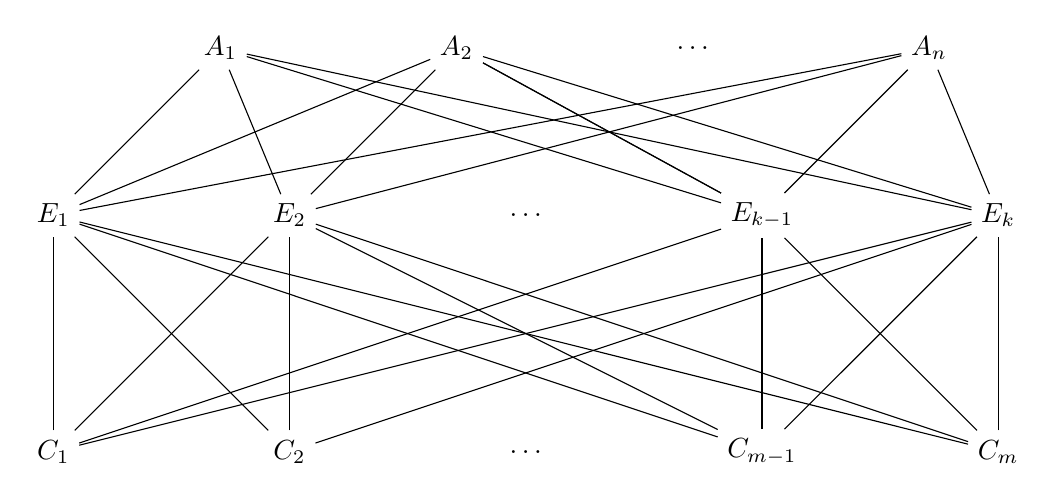
\begin{tikzpicture}[node distance={3cm}, main node/.style={draw, circle}]
  \node (a1) at (50, 1) {$A_1$};
  \node (a2) [right of=a1] {$A_2$};
  \node (dot) [right of=a2] {$\ldots$};
  \node (an) [right of=dot] {$A_n$};

  \node (e1) [below left of=a1] {$E_1$};
  \node (e2) [right of=e1] {$E_2$};
  \node (dot2) [right of=e2] {$\ldots$};
  \node (ek-1) [right of=dot2] {$E_{k-1}$};
  \node (ek) [right of=ek-1] {$E_k$};

  \node (c1) [below of=e1] {$C_1$};
  \node (c2) [right of=c1] {$C_2$};
  \node (dot3) [right of=c2] {$\ldots$};
  \node (cm-1) [right of=dot3] {$C_{m-1}$};
  \node (cm) [right of=cm-1] {$C_m$};

  \draw[-] (a1) to (e1);
  \draw[-] (a1) to (e2);
  \draw[-] (a1) to (ek-1);
  \draw[-] (a1) to (ek);

  \draw[-] (a2) to (e1);
  \draw[-] (a2) to (e2);
  \draw[-] (a2) to (ek-1);
  \draw[-] (a2) to (ek);

  \draw[-] (an) to (e1);
  \draw[-] (an) to (e2);
  \draw[-] (an) to (ek-1);
  \draw[-] (an) to (ek);

  \draw[-] (c1) to (e1);
  \draw[-] (c1) to (e2);
  \draw[-] (c1) to (ek-1);
  \draw[-] (c1) to (ek);

  \draw[-] (c2) to (e1);
  \draw[-] (c2) to (e2);
  \draw[-] (a2) to (ek-1);
  \draw[-] (c2) to (ek);

  \draw[-] (cm-1) to (e1);
  \draw[-] (cm-1) to (e2);
  \draw[-] (cm-1) to (ek-1);
  \draw[-] (cm-1) to (ek);

  \draw[-] (cm) to (e1);
  \draw[-] (cm) to (e2);
  \draw[-] (cm) to (ek-1);
  \draw[-] (cm) to (ek);
\end{tikzpicture}
\end{center}

Graph can also be correlation matrix - one for each VWAP, Open, Close, High, Low. Simpler, less assumptions, more computational resources required.

\newpage

\section*{Schedule:}

\begin{enumerate}
  \item Nov 22 - Nov 29:
    \begin{itemize}
      \item Find papers for 1) design of LSTM architecture 2) Technical indicators 3) Graph structure of data and best representation 4) design of GNN architecture
      \item Clean data as reasonable, organize as time-series feed of minute-by-minute states of the market
      \item Build data loading/preprocessing portion of training pipeline - can implement auto-encoder to condense features matrix into a vector embedding for LSTM?
      \item Implement LSTM model
    \end{itemize}
  \item Nov 29 - Dec 6:
    \begin{itemize}
      \item Start training LSTM model
      \item Implement graph model
      \item Train graph model/LSTM+GNN model as end-to-end
      \item Start write up of background
    \end{itemize}
  \item Dec 6 - Dec 13:
    \begin{itemize}
      \item Continued experiments
      \item Continue write up
    \end{itemize}
  \item Dec 13 - Dec 20: 
    \begin{itemize}
      \item Last experiments (hopefully none)
      \item Finish write up
    \end{itemize}
\end{enumerate}

\end{document}